\part{Classical Control Theory}

\chapter{Preliminaries}

\section{Euler's Identity} \label{Sec_Prelim_EulersIdentity}

Euler's number $e$ is a special number that is used in Euler's identity, it was originally discovered by Jacob Bernoulli from the problem of compound interest. Consider the formula for compound interest:
\begin{equation}
	A = P \left( 1 + \frac{r}{n} \right)^{nt}
\end{equation}
where,
\begin{itemize}
	\item A is the amount that is returned after interest
	\item P is the principle
	\item r is the interest rate
	\item n is the number of interest compounded per unit time
	\item nt is the total time of interest
\end{itemize}
Jacob Bernoulli wanted to know how much A would be maximized by making the interest maximum to $100\%$. He observed that no matter how much times the number of intervals $n$ was used, A never crossed a maximum value of $2.72$ for a P of $1$. The exact number is $2.71828182$ with more decimals following, Euler named this special number $e$ after his own name. 

One of the ways to calculate this special number $e$ using only basic mathematical operations (addition, subtraction, multiplication, division) is by using infinite series. $e$ can be calculated as follows:
\begin{align*}
	e	&= 1 = 1.00 \\
		&\approx 1 + \frac{1}{1!} = 2.00 \\
		&\approx 1 + \frac{1}{1!} + \frac{1}{2!} = 2.50 \\
		&\approx 1 + \frac{1}{1!} + \frac{1}{2!} + + \frac{1}{3!} = 2.666 \\
		&\approx 1 + \frac{1}{1!} + \frac{1}{2!} + + \frac{1}{3!} + \frac{1}{4!} = 2.708 \\
		&\approx 1 + \frac{1}{1!} + \frac{1}{2!} + + \frac{1}{3!} + \frac{1}{4!} + \frac{1}{5!} = 2.716
\end{align*}

As more terms are added into the infinite series, more accurate $e$ can be calculated. The advantage of infinite series is that it is easier to predict the next value of $e$ by adding factorials into the series. As a number, $e = 2.716$ from the infinite series can be written as $e^{1}$, in general $e$ can be raised to any number $x$ and therefore, the series can be written in the follow form for a general case:
\begin{equation}
	e^{x} = 1 + \frac{x}{1!} + \frac{x^{2}}{2!} +  \frac{x^{3}}{3!} + \frac{x^{4}}{4!} + \frac{x^{5}}{5!} + \cdot \cdot \cdot
\end{equation}

It can be seen that a smooth function (easily predictable) can be defined for $e$ using infinite series, other functions such as $sin(x)$ and $cos(x)$ are also smooth functions that can be easily determined using infinite series. For $sin(x)$ and $cos(x)$ the following series can be defined:
\begin{align}
	sin(x) &= \frac{x}{1!} - \frac{x^3}{3!} + \frac{x^5}{5!} - \frac{x^7}{7!} + \cdot \cdot \cdot \label{Eq_Prelims_sinx} \\ 
	cos(x) &= 1 - \frac{x^2}{2!} + \frac{x^4}{4!} - \frac{x^6}{6!} + \frac{x^8}{8!} \cdot \cdot \cdot \label{Eq_Prelims_cosx}
\end{align}

it seems that the Euler's number $e$ and the sum of $sin(x)$ and $cos(x)$ have some similarities except from the alternating signs that comes from the sum of $sin(x)$ and $cos(x)$ as shown below:
\begin{equation}
	sin(x) + cos(x) = 1 + \frac{x}{1!} - \frac{x^{2}}{2!} - \frac{x^{3}}{3!} + \frac{x^{4}}{4!} + \frac{x^{5}}{5!} - \frac{x^{6}}{6!} - \frac{x^{7}}{7!} \cdot \cdot \cdot
\end{equation}
The difference is in the sign of the following terms:
\begin{equation*}
	- \frac{x^{2}}{2!} \quad - \frac{x^{3}}{3!} \quad - \frac{x^{6}}{6!} \quad - \frac{x^{7}}{7!} \cdot \cdot \cdot
\end{equation*}
The idea is to multiply these terms with some number in such a way that when that number is square it produces a negative equal to $-1$. Such a number does not exits in reality, but because this number has to be included into the mathematics in order to further solve a problem, an imaginary number is invented such that $i^2 = -1$. This imaginary number was invented because this problem was occurring quite frequently in mathematics and such a number had to be imagined. Now with the invention of an imaginary number the infinite series for $e^{x}$ is now defined for $e^{ix}$, the following series will be produced:
\begin{equation} \label{Eq_Prelims_eix}
	e^{ix} = 1 + \frac{ix}{1!} + \frac{(ix)^2}{2!} + \frac{(ix)^3}{3!} + \frac{(ix)^4}{4!} + \frac{(ix)^5}{5!} + \frac{(ix)^6}{6!} + \frac{(ix)^7}{7!} \cdot \cdot \cdot
\end{equation}
Now,
\begin{itemize}
	\item $i^2 = -1$
	\item $i^3 = i^2 \times i = -i$
\end{itemize}
From equation \ref{Eq_Prelims_eix}:
\begin{equation*}
	e^{ix} = 1 + \frac{ix}{1!} - \frac{x^{2}}{2!} - \frac{ix^{3}}{3!} + \frac{x^{4}}{4!} + \frac{ix^{5}}{5!} - \frac{x^{6}}{6!} - \frac{ix^{7}}{7!} \cdot \cdot \cdot
\end{equation*}
Rearranging $i$ terms and all other terms:
\begin{equation} \label{Eq_Premilms_eix2}
	e^{ix} = \left(1 - \frac{x^{2}}{2!} + \frac{x^{4}}{4!} - \frac{x^{6}}{6!} + \frac{x^8}{8!} \right)
			+ i \left( \frac{x}{1!} - \frac{x^{3}}{3!} + \frac{x^{5}}{5!} - \frac{x^{7}}{7!} \right)
\end{equation}
comparing equation \eqref{Eq_Premilms_eix2} with equations \eqref{Eq_Prelims_sinx} and \eqref{Eq_Prelims_cosx}, it can be seen that:
\begin{equation} \label{Eq_Prelims_EulersFormula}
	e^{ix} = cos(x) + i sin(x)
\end{equation}
Equation \eqref{Eq_Prelims_EulersFormula}, is called the \textbf{\textit{Euler's Formula}}. A special case of Euler's formula leads to \textbf{\textit{Euler's Identity}}, which occurs when $e^{ix} = e^{i\pi}$. Consider equation \eqref{Eq_Prelims_EulersFormula}, since $cos(\pi)$ = -1 and $sin(\pi) = 0$, Euler's formula now reduces to:
\begin{equation} \label{Eq_Prelims_EulersIdentity}
	e^{i\pi} = -1 + i 0 \implies e^{i\pi} + 1 = 0
\end{equation}
Equation \eqref{Eq_Prelims_EulersIdentity}, relates four mathematical concepts in one formula which are:
\begin{itemize}
	\item Euler's number $e$
	\item cosine and sine terms
	\item Irrational number $\pi$
	\item Complex number $i$
\end{itemize}

\section{Linear differential equations} \label{Sec_Prelim_LDE}

The input/output behavior of a system can be described using linear differential equation:
\begin{equation} \label{Eq_Prelim_LDE}
	\frac{d^{n}y}{dt^{n}} + a_1 \frac{d^{n-1}y}{dt^{n-1}} ... + a_n y = b_1 \frac{d^{n-1}u}{dt^{n-1}} ... + b_n u
\end{equation}
where, $y$ and $u$ are number of inputs and outputs of the system respectively and $a_k$ and $b_k$ are real constant coefficients. For all such linear differential equations, the solution of the differential equation \eqref{Eq_Prelim_LDE} is expressed as a linear combination of \textbf{\textit{null solution}} and \textbf{\textit{particular solution}} as
\begin{equation}
	y(t) = y_{n}(t) + y_{p}(t)
\end{equation}

\subsection{Null Solution}

the null solution is the function of system variables $y(t)$ (when input to the system is zero) and particular solution is the function of inputs to the system $u(t)$. The null solution $y_{n}$ is derived from its characteristic equation, the null solution is then a linear combination of the roots of the characteristic equation. Therefore, if the roots of the characteristic equation are $s_k$, it forms that
\begin{equation} \label{Eq_Prelim_NullSolution}
	y_{n}(t) = \sum_{k = 1}^{n} C_{k} e^{s_{k}t}
\end{equation} 
The characteristic equation of an differential equation (such as equation \eqref{Eq_Prelim_LDE} when RHS is zero) with the roots $s_{k}$ is given as
\begin{equation} \label{Eq_Prelim_CharacteristicEquation}
	a(s) = s^{n} + a_1 s^{n-1} + ... + a_n = 0
\end{equation} 
The solution depends on the number of roots and the number of roots depends on the order of the characteristic equation \eqref{Eq_Prelim_CharacteristicEquation}. Using the derived roots of characteristic equation \ref{Eq_Prelim_CharacteristicEquation} $(s_{k})$, the terms $\sum_{k = 1}^{n} e^{s_{k}t}$ of the null solution can be found. The parameter $C_k$ is dependent on the initial conditions of the system, they are included there to include the IC's.

\subsubsection{Deriving characteristic equation for LDE}

Lets consider the solution of the LDE \ref{Eq_Prelim_LDE} is given by a smooth sinusoidal function 
\begin{equation} \label{Eq_SmoothFunction}
	y(t) = e^{st}
\end{equation}
substituting equation \eqref{Eq_SmoothFunction} into LDE \ref{Eq_Prelim_LDE} (inputs are ignored to find characteristic equation)
\begin{equation} 
	s^{k}e^{st} + a_1 s^{k-1}e^{st} ... + a_n e^{st} = 0 \implies (s^{k} + a_1 s^{k-1} ... + a_n) e^{st} = 0
\end{equation}
since $e^{st}$ cannot be a zero, there the term $s^{k} + a_1 s^{k-1} ... + a_n$ should diminish to zero. Therefore, the characteristic equation of \ref{Eq_Prelim_LDE} is given by
\begin{equation} \label{Eq_CharacteristicEqLDE}
	s^{k} + a_1 s^{k-1} ... + a_n = 0
\end{equation}
The roots of this characteristic equation \eqref{Eq_CharacteristicEqLDE} depends on the order of the LDE. For second order systems, the characteristic equation becomes quadratic and is expressed by
\begin{equation}
	s^{2} + a_{1}s + a_{2} = 0 
\end{equation}
with the roots $s_{1,2}$ therefore being quadratic.

\subsection{Particular Solution}
\newpage
The process of finding the particular solution can be visualized using the figure \ref{Fig_Pre_Flow_LDE_Sol_using_LT}.
\begin{figure}[h!]
	\centering
	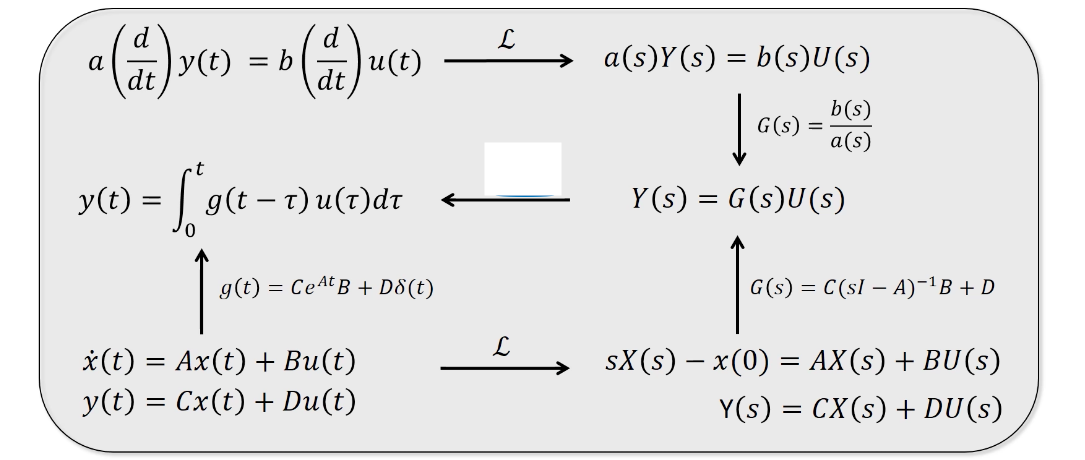
\includegraphics[width=\linewidth]{Bilder/Solutiion_of_LDE_4m_LT}
	\caption{Flow of solution to LDE to and from Laplace Transforms}
	\label{Fig_Pre_Flow_LDE_Sol_using_LT}
\end{figure}

As a particular solution depends on the input, lets consider a sinusoidal input such that $ u(t) = e^{st}$, where $s$ is a complex number $s = \sigma + j \omega$ and $\sigma$ is chosen such that the input signal is a damped signal. An investigation can be performed to check if there is a unique particular solution of the form
\begin{equation} \label{Eq_Prelim_ParticularSolution}
	y(t) = G(s)u(t) \implies y(t) = G(s)e^{st}
\end{equation}
Equation \eqref{Eq_Prelim_ParticularSolution} is chosen such that the solution $y(t)$ is some function $G(s)$ of the input signal $y(t)$. The idea is to determine this unknown function $G(s)$, the following steps deals with determining $G(s)$. 

Substituting equation \eqref{Eq_Prelim_ParticularSolution} into the differential equation \eqref{Eq_Prelim_LDE} and writing its characteristic equation gives:
\begin{equation}\label{Eq_Prelim_ParticularSolution_2}
	(s^{n} + a_1 s^{n-1} + ... + a_n)G(s)e^{st} = (b_{1}s^{n-1} + ... + b_n)e^{st}
\end{equation}
From equation \eqref{Eq_Prelim_ParticularSolution_2}, it can be seen that $G(s)$ can be determined as the ratio of two polynomials on LHS and RHS which here are labeled as $b(s)$ and $a(s)$ respectively
\begin{equation}\label{Eq_Prelim_TransferFunction}
	G(s) = \frac{b_{1}s^{n-1} + ... + b_n}{s^{n} + a_1 s^{n-1} + ... + a_n} = \frac{b(s)}{a(s)}
\end{equation}
Equation \eqref{Eq_Prelim_TransferFunction} is called the \textbf{\textit{Transfer function}}. A Transfer function is the ratio of output to the input of a system.

Now, the solution to the differential equation is expressed as the linear combination of equations \eqref{Eq_Prelim_NullSolution} and \eqref{Eq_Prelim_ParticularSolution}
\begin{equation} \label{Eq_Prelim_SolutionLDE}
	y(t) = \sum_{k = 1}^{n} C_{k} e^{s_{k}t} + G(s)e^{st}
\end{equation}
the first term in equation \eqref{Eq_Prelim_SolutionLDE} is due to the IC's and the second term is due to the inputs via transfer function.

The \textbf{\textit{Transfer function}} $G(s)$ can be determined using Laplace Transform. Notice, however, in this example we did not use LT to find the particular solution so no inverse LT can be performed to determine the transfer function $G(s)$. In this case therefore, the step of writing the particular solution as a convolutional integral term in time domain cannot be done. 

The solution to LDE using figure \ref{Fig_Pre_Flow_LDE_Sol_using_LT} is given here to indicate that particular solutions contain transfer function and this can be found easily using Laplace transforms instead.

\subsection{Laplace transform}

The transfer function as given by equation \eqref{Eq_Prelim_TransferFunction} can be determined using Laplace transform. The LT for a function $f(t)$ written in time domain is generally defined in $s$-domain as
\begin{equation}
	F(s) = \mathcal{L}\{f(t)\} = \int_{0}^{\infty} f(t) e^{-st} dt
\end{equation}
Where $f(t)$ is transformed into $s$-domain using the above definition. Here $s$ is called a Laplace variable and is complex in nature. For a differential in time-domain, in LT the equivalent is multiplication with Laplace variable $s$ and subtraction with initial conditions such that
\begin{equation}
	\mathcal{L}\{\frac{df(t)}{dt}\} = sF(s) - f(0)
\end{equation}
If the system is originally at rest at $t = 0$ such all IC's are zero, then the transfer function of a differential equation \eqref{Eq_Prelim_LDE} can be expressed as the ratio of outputs to inputs
\begin{equation} \label{Eq_Prelim_Random1}
	Y(s) = \frac{b_{1}s^{n-1} + ... + b_n}{s^{n} + a_1 s^{n-1} + ... + a_n} U(s) = \frac{b(s)}{a(s)} U(s) = G(s) U(s)
\end{equation}
Laplace transform follows the \textbf{\textit{convolution theory}} such that the solution from the product of two equations in time domain is individual terms taken in Laplace domain as
\begin{equation}
	\mathcal{L} \left\{ \int_{0}^{t} g(t - \tau) f(t) d\tau \right\} = \mathcal{L} \{ g(t) \} \mathcal{L} \{ f(t) \} = G(s)F(s)
\end{equation}
using the above result, the solution to equation \eqref{Eq_Prelim_Random1} (replace $F(s)$ with $U(s)$) can be determined easily for any input signals $U(s)$ as the following relationships holds good in the Laplace domain:
\begin{equation} \label{Eq_Prelim_ConvolutionalIntegral}
	\mathcal{L} \left\{ \int_{0}^{t} g(t - \tau) u(t) d\tau \right\} = G(s)U(s)
\end{equation}

The transfer function $G(s)$ can actually be used to express the systems response to an arbitrary input signal.

\textbf{\textit{Note: }} the term $g(t)$ in the convolutional integral is the impulse response and $u(t)$ is the input signal. Therefore, using convolutional integral the solution $y(t)$ can be convoluted using the solution of $g(t)$ to any input signal $u(t)$.

\section{Example of solving a LDE} \label{Sec_Prelim_LDE_Ex}

Lets consider a LDE given as
\begin{equation} \label{Eq_Prelim_Ex_LDE}
	\dot{x} = a x + b u, \quad x(0) = x_0
\end{equation}
\textbf{\textit{Null Solution}} \\
For null solution we have to first find the characteristic equation, assuming a solution with a smooth function such that $x(t) = C e^{st}$, the characteristic equation can be found by substituting $x(t) = C e^{st}$ into equation \eqref{Eq_Prelim_Ex_LDE} and considering terms with $u = 0$
\begin{equation}
	\dot{x} - ax = 0 \implies C s e^{st} - C a e^{st} = 0 \implies C e^{st} (s - a) = 0 \implies s - a = 0
\end{equation}
the root of characteristic equation is $s = a$, substituting this in equation $x(t) = C e^{st}$
\begin{equation}
	x_{n}(t) = C e^{at}
\end{equation}
where $C$ can be found from IC
\begin{equation}
	x_{n}(0) = C e^{a 0} = x_0 \implies C = x_0
\end{equation}
which completes the null solution
\begin{equation} \label{Eq_Prelim_LDE_Ex_NullSolution}
	x_{n} = x_0 e^{at}
\end{equation}
\textbf{\textit{Particular Solution}} \\
The particular solution can be found using the convolutional integral \eqref{Eq_Prelim_ConvolutionalIntegral}, in order to use the convolutional integral we first need the impulse response. The impulse response can be in-turn written using inverse LT of the TF
\begin{equation*}
	g(t) = \mathcal{L}{G(s)}
\end{equation*}

starting from LT of equation \eqref{Eq_Prelim_Ex_LDE}
\begin{equation}
	\mathcal{L} \{ \dot{x} = a x + b u \} \implies s X(s) - x_0 - a X(s) = b U(s)
\end{equation}
further transfer function needs that the IC's are zero,
\begin{equation}
	X(s) (s - a) = b U(s) \implies G(s) = \frac{X(s)}{U(s)} = \frac{b}{s - a} 
\end{equation}
the solution in Laplace domain can be written as
\begin{equation}
	X(s) = G(s)U(s)
\end{equation}
finally, $g(t)$ can be found from inverse LT to write the solution $x(t)$ in time-domain 
\begin{equation}
	\mathcal{L}^{-1} \{ G(s) \} = \mathcal{L}^{-1} \left\{\frac{b}{s-a}\right\} = b e^{at}
\end{equation}
the complete particular solution due to an input $u(t)$ is therefore derived from the convolutional integral
\begin{equation} \label{Eq_Prelim_LDE_Ex_ParticularSolution}
	x_p = \int_{0}^{t} g(t - \tau) u(\tau) d\tau = \int_{0}^{t} b e^{a(t - \tau)} u(\tau) d\tau
\end{equation}
where $\tau$ is a constant in time when $u$ is applied. The complete solution to equation \eqref{Eq_Prelim_Ex_LDE} is therefore given by
\begin{equation} \label{Eq_Prelim_LDE_Ex_FullSolution}
	x(t) = x_{n}(t) + x_{p}(t) = x_0 e^{at} + \int_{0}^{t} b e^{a(t - \tau)} u(\tau) d\tau
\end{equation}

\section{Basic definitions of Linear system}

A system is linear with respect to its inputs and outputs if and only if (iff) \textbf{\textit{superposition}} hold. Principle of superposition says that if there are two inputs $u_1$ and $u_2$ which produce outputs $y_1$ and $y_2$ respectively, then the total response of the system from these two inputs can be determined as a linear combination of two outputs as
\begin{equation}
	y = a u_1 + b u_2
\end{equation}
It also says that the amplitudes $a$ and $b$ do not matter, if we scale inputs by factors $a$ and $b$ respectively, the outputs also scale individually as shown in the equation above.

A \textbf{\textit{linear time-invariant}} system is independent of time such that the coefficients $(a_k \quad b_k)$ of the differential equation \eqref{Eq_Prelim_LDE} are constant. If the coefficients become dependent on time, then equation \eqref{Eq_Prelim_LDE} become time-variant (ie., the response changes as time of application of inputs changes).

\section{Solution to differential of $e^{\lambda t}$}

The value of $e^{\lambda t}$ where $\lambda$ is a scalar, can be found using infinite series and can be expressed as the sun
\begin{equation}
	e^{\lambda t} := \sum_{k = 0}^{\infty} \frac{(\lambda t)^{k}}{k!}
\end{equation}
taking the time derivative
\begin{equation}
	\frac{d}{dt} e^{\lambda t} = \frac{d}{dt} \left( \sum_{k = 0}^{\infty} \frac{(\lambda t)^{k}}{k!} \right)
\end{equation}
Note that the infinite series can be expanded from second to the infinite term as follows
$$ e^{\lambda t} = 1 + \sum_{k = 1}^{\infty}  \frac{(\lambda t)^{k}}{k!} $$
using the above result, the derivative of constant can be removed from the original equation, leaving behind the derivative from second to the infinite term. Also note that the derivative $\frac{d}{dt} ((\lambda t)^{k})$ is of the form $\frac{d}{dt} (x^{n}) := n x^{n -1}$
\begin{equation}
	\frac{d}{dt} e^{\lambda t} = \lambda \sum_{k = 1}^{\infty} \frac{k (\lambda t)^{k - 1}}{k!}
\end{equation}
the term $k$ in the numerator cancels the term $k$ in the denominator leaving behind the factorial $(k-1)!$, the differential now becomes
\begin{equation}
	\frac{d}{dt} e^{\lambda t} = \lambda \sum_{k = 1}^{\infty} \frac{(\lambda t)^{k - 1}}{(k-1)!}
\end{equation}
if we substitute a ne coordinate $l$ such that $l = (k-1)$, the infinite series becomes
\begin{equation}
\frac{d}{dt} e^{\lambda t} = \lambda \sum_{l = 0}^{\infty} \frac{(\lambda t)^{l}}{l!}
\end{equation}
which again is the definition of the infinite series $e^{\lambda t}$, therefore, the solution to the differential now becomes
\begin{equation}
	\frac{d}{dt} e^{\lambda t} = \lambda e^{\lambda t}
\end{equation}

\section{Solution to differential of an exponential matrix $e^{\vec{A} t}$} \label{Sec_Prelims_solution_matrix_exp}

\subsection{Defining $e^{\vec{A} t}$}
If $\vec{A}$ is to be diagonal, then it is defined as 
\begin{equation}
	e^{\vec{A}t} = \vec{E}\vec{\Lambda}\vec{E}^{-1}
\end{equation}
where,
\begin{equation}
	\lambda = \begin{bmatrix}
	\lambda_{1} & 0 \\ 0 & \lambda_{2}
	\end{bmatrix}
\end{equation}

Using the definition above for $\vec{A}$, the exponential with matrix $\vec{A}$ can be defined as
\begin{equation}
	e^{\vec{A}t} = \sum_{k = 0}^{\infty} \frac{1}{k!}(\vec{E}\vec{\Lambda}\vec{E}^{-1} t)^{k}
\end{equation}
simplifying the above equation
\begin{equation}
	e^{\vec{A}t} = \sum_{k = 0}^{\infty} \frac{1}{k!} (\vec{E})^{k} (\vec{\Lambda})^{k} (\vec{E}^{-1})^{k} t^{k}
\end{equation}
Apparently the terms $\vec{E}$ and $\vec{E}^{-1}$ can be factored out leaving the terms $\vec{\Lambda}^{k} t^{k}$ inside the summation
\begin{equation}
	e^{\vec{A}t} = \vec{E} \left(\sum_{k = 0}^{\infty} \frac{1}{k!} (\vec{\Lambda} t)^{k} \right) \vec{E}^{-1}
\end{equation}
further,
\begin{equation}
e^{\vec{A}t} = \vec{E} \left(\sum_{k = 0}^{\infty} \frac{1}{k!} \begin{bmatrix}
	(\lambda_{1} t)^{k} & 0 \\ 0 & (\lambda_2 t)^{k}
\end{bmatrix} \right) \vec{E}^{-1}
\end{equation}
Now the terms inside the summation is the definition of exponential for every diagonal element, therefore,
\begin{equation}
	e^{\vec{A}t} = \vec{E} \begin{bmatrix}
	e^{\lambda_{1}t} & 0 \\ 0 & e^{\lambda_{2} t}
	\end{bmatrix} \vec{E}^{-1}
\end{equation}
Therefore, it can be said that \textbf{\textit{exponent of a diagonal matrix}} is a \textbf{\textit{exponent of diagonal elements}}.

\subsection{Time derivative of exponential matrix $e^{\vec{A} t}$} \label{Sec_1_ch_1_ddtOfMatrixExp}

using the definition
\begin{equation}
e^{\vec{A}t} = \sum_{k = 0}^{\infty} \frac{1}{k!}(\vec{E}\vec{\Lambda}\vec{E}^{-1} t)^{k}
\end{equation}
time-derivative is expressed as
\begin{align*}
	\frac{d}{dt} e^{\vec{A}t} &= \frac{d}{dt} \left(\sum_{k = 0}^{\infty} \frac{1}{k!}(\vec{E}\vec{\Lambda}\vec{E}^{-1} t)^{k}\right) \\
							&= \frac{d}{dt} \left(\vec{E} \left(\sum_{k = 0}^{\infty} \frac{1}{k!} (\vec{\Lambda} t)^{k} \right) \vec{E}^{-1}\right) \\
							&= \frac{d}{dt} \vec{E} \left(\begin{bmatrix}
								1 & 0 \\ 0 & 1
							\end{bmatrix} + \sum_{k=1}^{\infty} \frac{1}{k!}(\Lambda t)^{k} \right) \vec{E}^{-1} \\
							&= \sum_{k=1}^{\infty} \frac{1}{(k - 1)!} \vec{E} \begin{bmatrix}
								(\lambda_{1} t)^{k-1} & 0 \\ 0 & (\lambda_{2} t)^{k-1}
							\end{bmatrix} \vec{E}^{-1} \\
							&= \vec{A}e^{\vec{A}t}
\end{align*}

\subsection{State Transition Matrix}
The solution from section \ref{Sec_1_ch_1_ddtOfMatrixExp} that the matrix exponential behaves same like a scalar exponential is central in Control theory and appears so often in LTI systems, it is given its own name and called as a \textbf{\textit{State Transition Matrix}} and is denoted using a special symbol as shown,
\begin{equation}
	e^{\vec{A}(t - t_{0})} = \Phi(t, t_{0})
\end{equation}

This helps establish the following results, suppose a time derivative of a matrix exponential is to be determined, as it is known that a  matrix exponential behaves same like a scalar exponential, it can be said that,

if the time-derivative of a scalar exponential is given as follows
\begin{equation}
	\frac{d}{dt}e^{at} = a e^{at}
\end{equation}
then the time-derivative of a matrix exponential is given as follows
\begin{equation}
\frac{d}{dt}e^{At} = \frac{d}{dt}\Phi(t, t_{0}) = A \Phi(t, t_{0})
\end{equation}
and also it can be proven that,
\begin{equation}
	\Phi(t, t) = \vec{I}
\end{equation}
where $\vec{I}$ is the Identity matrix. As substituting $t_{0} = t$ will make the matrix exponential $e^{0} = 1$.

\subsection{Solutions to free and forced response of a system using results from State Transition Matrix}
\subsubsection{Null Solution}
As the solution to $\frac{d}{dt}e^{At}$ is given by
\begin{equation} \label{Eq_1_ch_1_STM_NullSolution}
	\frac{d}{dt}e^{At} = \frac{d}{dt}\Phi(t, t_{0}) = A \Phi(t, t_{0})
\end{equation}
comparing \eqref{Eq_1_ch_1_STM_NullSolution} with a state-space model,
$$\dot{\vec{x}} = \vec{A}x + \vec{B}u$$ $\vec{A}x$ forms the solution when there are no inputs to the system. Equation \eqref{Eq_1_ch_1_STM_NullSolution} denotes the null solution to the time-derivative of a State Transition Matrix.

\subsubsection{Particular Solution}
In mathematics, the solution to the time-derivative of a State Transition Matrix with a given input $u$ $(\dot{x} = Ax + Bu)$ is expressed as
\begin{equation} \label{Eq_1_ch_1_STM_ParticularSolution}
	x(t) = \Phi(t, t_{0}) x(t) + \int_{t_{0}}^{t} \Phi(t, \tau) \vec{B}u(\tau)d\tau
\end{equation}
where $\tau$ is a dummy integral variable used to to plug in any required value of $t$. The term with integral is called constitutional integral term. The plausibility that \eqref{Eq_1_ch_1_STM_ParticularSolution} is a unique solution to the time-derivative of a State Transition Matrix with an input $u$ can be checked using \textbf{\textit{Initial Condition check}} and \textbf{\textit{Dynamics check}}.

\textbf{\textit{Initial Condition check}}
Initial Condition check can be done by substituting $t = t_{0}$, therefore \eqref{Eq_1_ch_1_STM_ParticularSolution} becomes
\begin{equation} 
x(t_{0}) = \Phi(t, t_{0}) x(t_{0}) + \int_{t_{0}}^{t_{0}} \Phi(t_{0}, \tau) \vec{B}u(\tau)d\tau
\end{equation}
where $\Phi(t_{0}, t_{0}) = \vec{I}$ as established earlier and the term with integral goes to zero. Leaving behind the solution
\begin{equation} 
x(t) = \vec{I} x(t_{0})
\end{equation}

\section{Why Eigenvalue Analysis}

Consider a linear system of ODE $$\dot{x} = Ax$$ where $x$ is a vector in the space $\mathbb{R}^{n}$. The solution of this ODE is $$x(t) = e^{At}x(0)$$ The dynamics of this system is dependent on the solution of $e^{At}$ which needs to the solved analytically in order to determine the solution of this ODE. One of the solution is using Taylor series expansion of the exponential and then plugging the matrix $A$ into the expansion, the series is expressed as
\begin{equation}
	e^{At} = I + \frac{At}{1!} + \frac{A^{2}t^{2}}{2!} +  \frac{A^{3}t^{3}}{3!} + ...
\end{equation}

the problem with this solution is that since $A$ is a matrix computing this expression every time to determine the solution to the ODE would be a daunting task. Therefore, in mathematics, the solution was determined to use some-other arbitrary vector $\xi$ which is coordinate transformed from the actual vector $x$ such that computing the solution in that coordinate transformed vector $\xi$ would be fairly straight forward and easier.

In actual practice, eigenvalues and Eigen vectors of $A$ are used to get a coordinate transformation from $x$ coordinate to some eigenvector coordinate where it is easier to write the solution to $e^{At}$.

\subsection{Eigenvalues and Eigenvectors}

In general, eigenvalues and eigenvectors satisfy the following relation
\begin{equation}\label{eq_0_ch_0_ev_ev0}
	A \xi = \lambda \xi
\end{equation}
where $\lambda$ is a scalar, this is because when $\xi$ is multiplied by $A$, it still remains the original vector $\xi$ pointing in the same direction though its length gets scaled or it might be flipped to negative direction. This is scaling of a vector and therefore, the above relationship that $\xi$ get scaled to a scalar quantity $\lambda$. 

Note*** In general, a matrix coordinate transforms a vector and a scalar scales a vector.

Note*** here $\xi$ is a special vector where this relationship is true that $A \xi = \lambda \xi$, this is possible for a limited special case, not every time.

Lets denote a vector $T$ which contains all the $\xi$ such that $T = \xi$ and expressed as
$$T = [\xi_1 \quad \xi_2 \quad \xi_3 \quad ... \xi_n]$$ and consider another $D$ which is a diagonal matrix of $\lambda$ such that
$$\begin{bmatrix}
\lambda_{1} & 0 & 0 \\ 0 & \lambda_{2} & 0 \\ 0 & 0 & \lambda_{3}
\end{bmatrix}$$
assume that the matrix $D$ is extended upto the dimension $(n\times n)$. Now using these defined matrices, the new definition of eigenvalues and eigenvectors can be expressed as
\begin{equation}\label{eq_0_ch_0_ev_ev1}
	AT = TD
\end{equation}
Now the reason for writing eigenvalues and eigenvectors is because using this system and using coordinate transform, the vector $x$ which is represented in some arbitrary coordinate system is transformed to the coordinate system when $\xi$ exists where things get simpler. The transformation is expressed as
$$x = Tz$$ where $T$ is an invertible matrix which when multiplied by another arbitrary coordinate $z$ represents the coordinate transform of $x$. Therefore, the new dynamics in the $z$ coordinate can be expressed as
\begin{equation}
	\dot{x} = T\dot{z} \implies T\dot{z} = Ax \implies  T\dot{z} = ATz
\end{equation}
it follows that
\begin{equation}\label{eq_0_ch_0_ev_ev2}
	\dot{z} = T^{-1}ATz
\end{equation}
from equation \eqref{eq_0_ch_0_ev_ev1} it follows that
\begin{equation}
	T^{-1}AT = D
\end{equation}
therefore, using \eqref{eq_0_ch_0_ev_ev1} and \eqref{eq_0_ch_0_ev_ev2}
\begin{equation}\label{eq_0_ch_0_ev_ev3}
	\dot{z} = Dz
\end{equation}
here, \eqref{eq_0_ch_0_ev_ev3} is similar in form as \eqref{eq_0_ch_0_ev_ev0} which is also a linear dynamical system. The one thing that is nice about this new representation \eqref{eq_0_ch_0_ev_ev3} is that here, $D$ is a diagonal matrix instead of $A$ which was not. The advantage that a diagonal matrix $D$ has over a general matrix like $A$ is that with $D$ all the dynamics gets decoupled such that each term of the state dynamics $dot{z}_{i}$ is only related to each of the $z_{i}$ coordinate, so the dynamics have been unpacked to their most simplest form with their coordinates using this transformed coordinate $z$. Consider the following expression
\begin{equation}
	\frac{d}{dt}\begin{bmatrix}
		z_{1} \\ z_{2} \\ . \\ . \\ . \\ z_{n}
	\end{bmatrix} = \begin{bmatrix}
		\lambda_{1} & 0 & 0 & ... & 0 \\ 0 & \lambda_{2} & 0 & ... & 0 \\ 0 & 0 & \lambda_{3} & ... & 0 \\ . \\. \\. \\ 0 & 0 & 0 & ... & \lambda_{n}
	\end{bmatrix}\begin{bmatrix}
	z_{1} \\ z_{2} \\ . \\ . \\ . \\ z_{n}
	\end{bmatrix}
\end{equation}
The solution of this diagonal matrix is a special case in mathematics as each of the scalar diagonal terms have the following solution for the equation $\dot{z} = Dz$
\begin{equation}
	z(t) = e^{Dt}z(0) = \begin{bmatrix}
		e^{\lambda_{1} t} & 0 & 0 & ... & 0 \\ 0 & e^{\lambda_{2} t} & 0 & ... & 0 \\ 0 & 0 & e^{\lambda_{4} t} & ... & 0 \\ . \\. \\. \\ 0 & 0 & 0 & ... & e^{\lambda_{n} t}
	\end{bmatrix}z(0)
\end{equation}
such a solution is quite straight forward and simple compared to the solution of $e^{At}$ where the solution was given by a Taylor's series expansion. Using Matlab'S fucntion \textbf{\textit{[T,D] = eig(A);}} the transformation matrix $T$ and the diagonal matrix $D$ can be determined.

\subsection{Mapping matrix exponential to diagonal exponential}

From \eqref{eq_0_ch_0_ev_ev1}, matrix $A$ can be expressed as
\begin{equation}
	A = TDT^{-1}
\end{equation}
substituting this result in the Taylors expansion series
\begin{align*}
	e^{At} = e^{TDT^{-1}} &= TT^{-1} + TDT{-1}t + (TDT^{-1}TDT^{-1})\frac{t^{2}}{2!} + ... \\
						  &= T[I + Dt + \frac{D^{2}t^{2}}{2!} + \frac{D^{3}t^{3}}{3!}+ ...]T^{-1}
\end{align*}
\begin{equation}
	e^{At} = T e^{Dt} T^{-1}
\end{equation}

\section{Newton's Law's for rotating bodies}

Stating Newton's Law's for rotating bodies:
Starting from linear momentum, it is described as 
\begin{equation}
\vec{P_{/O}} = m \vec{v_{G_{/O}}}
\end{equation}
Where $\vec{P_{/O}}$ is the linear momentum expressed with reference to frame-O (Inertial frame). Linear momentum is always expressed in inertial frame-O, $v_{G}$ is the velocity of center of mass of the body. Further, from Newton's second law it can be seen that, the law states the rate of change of $\vec{P_{/O}}$ as
\begin{equation}
\sum \vec{F} = \frac{d}{dt}\vec{P_{/O}}
\end{equation}
However, the angular momentum itself is expressed as the moment of the moment, that is
\begin{equation}\label{Eq_Prelims_AnularMomentumDef}
\vec{H_{/A}} = \sum_{i}^{} r_{i_{/A}} \times p_{i_{/O}}
\end{equation}
where $\vec{H_{/A}}$ denotes angular momentum with reference to frame-A, $r_{i_{/A}}$ denotes the distance vector of body $i$ with reference to frame-A's origin. Because angular momentum unlike linear moment can be expressed with reference to any point of frame. So choosing an arbitrary frame $A$ so as to include any effects of off-the axis loading in the rotary system. Further, \eqref{Eq_Prelims_AnularMomentumDef} can be solved and expressed for solid bodies as
\begin{equation} \label{Eq_Prelims_AngularMomentumFormula}
	\vec{H_{/A}} = \vec{H_{/G}} + r_{G_{/A}} \times \vec{P_{/O}}
\end{equation}
the above equation can be written in pseudo-code as
\textbf{\textit{Angular momentum w.r.t any point A = Angular momentum w.r.t G + momentum due to off the axis loading of the rigid body from its 'G'}}

Here Frame-A is any moving frame w.r.t Inertial Frame-O, therefore, there will always be a term that calculates the angular momentum of $G$ w.r.t this moving frame. Alternatively, angular momentum can be calculated using matrix formula
\begin{equation} \label{Eq_Prelims_AngularMometumMatrixForm}
	\vec{H_{/A}} = [I_{/A}] \begin{bmatrix}
	\omega_{x} \\ \omega_{y} \\ \omega_{z}
	\end{bmatrix}
\end{equation}
However, using equation \eqref{Eq_Prelims_AngularMomentumFormula} the use of parallel-axis theorem to calculate the inertia tensor $[I_{/A}]$ can be avoided.

Finally, the net torques acting on the system can be calculated using Newton-Euler's equations for rotating rigid bodies
\begin{equation}
	\sum \mathcal{T_{/A}} = \frac{d}{dt}\vec{H_{/A}} + \vec{v_{A/O}} \times P_{/O}
\end{equation}
Similar, to angular momentum, if torques are to be calculated w.r.t to a moving Frame-A, then there will be an additional term to include the torques due to this moving frame.


\section{Harmonic Oscillator}

This section describes mathematical modeling of harmonic oscillator both its free and forced response. The forced response is 